% Template for FPL 2012 papers; to be used with:
%          spconf.sty   - ICASSP/ICIP LaTeX style file
%          IEEEtran.bst - IEEE bibliography style file

% Created:  Apr-May 2005 - Riku Uusikartano -- riku.uusikartano@tut.fi
% Modified: March-2012 - Daniel Mu�oz Arboleda -- damuz@unb.br
%
% Modified: April-2017 - Joao Guimaraes	-- joaoguimaraes31@gmail.com
% --------------------------------------------------------------------------

\documentclass[12pt,a4paper]{article}

\usepackage{fixos/spconf}
\usepackage{amsmath,epsfig}
\usepackage[brazilian]{babel} % Suporte para o Portugu�s
\usepackage[latin1]{inputenc} % Suporte para acentua��o sem necessidade dos comandos especiais.
\usepackage[]{subfigure}
\usepackage[portuguese,algoruled,longend]{algorithm2e}
\usepackage{multirow}
\usepackage{tabularx}
\usepackage{adjustbox}
\usepackage{graphicx}
\usepackage{titling}
\usepackage{dblfloatfix}
\usepackage{fancyhdr,floatpag}
\usepackage{steinmetz}
\usepackage[margin=3cm]{geometry}

% Titulo do documento
\title{Relat\' orio do Experimento 4}

%Disciplina
\newcommand{\disciplina}{Laborat\' orio de Eletricidade Aplicada}

%nome do autor
\author{Jo\~ ao Victor Avancini Guimar\~ aes}

%matricula
\newcommand{\matricula}{12/0122405}

%professor
\newcommand{\professor}{Rudi Van Els}

%data (em branco escreve data do dia)
\date{}


%%pages line numbers
\pagestyle{fancy}
\fancyhf{}% Clear page header/footer
\renewcommand{\headrulewidth}{0pt}% No header rule
\fancyfoot[C]{\thepage}
\floatpagestyle{fancy}
\pagenumbering{arabic}


\hyphenation{Tam-pe-re ela-bo-ra-cao}


\begin{document}
\begin{titlepage}

\newcommand{\HRule}{\rule{\linewidth}{0.5mm}} % Defines a new command for the horizontal lines, change thickness here

\center % Center everything on the page

\textsc{\LARGE \disciplina{}}\\[1.5cm] 
\textsc{\Large Universidade de Bras\' ilia}\\[0.5cm]

\vspace{3cm}


\HRule \\[0.4cm]
{ \huge \bfseries \thetitle }\\[0.4cm] % Title of your document
\HRule \\[1.5cm]
 

\vspace{2cm}


\textsc{\LARGE \theauthor }\\[0.8cm]
\textsc{\LARGE \matricula{} }\\[1.5cm]

\vspace{0.5cm}

\textsc{\Large \textit{Professor: } \professor{}}\\[1cm]


{\large \today}\\[2cm] % Date, change the \today to a set date if you want to be precise

%university logo
\begin{figure}[!b]
    \centering
    
\includegraphics[width=\linewidth]{images/logofgaunb.jpg}
\end{figure}


\vfill %fill the rest of the page with black space

\end{titlepage}


\tableofcontents
\newpage

\section{Introdu��o}
Circuitos lineares reagem diferentemente em corrente alternada e corrente cont�nua, naturalmente � mais f�cil analisar circuitos que trabalham com corrente cont�nua visto que elementos passivos armazenadores de energia como capacitores e indutores podem ser substituidos por curto-circuitos e circuitos abertos respectivamente. Um m�todo conveniente para analisar circuitos � o m�todo do Equivalente de Theven�n, o mesmo permite substituir uma rede linear complexa por um circuito composto por uma fonte de tens�o em s�re com uma imped�ncia. Para o c�lculo da fonte de tens�o de theven�n basta medir a tens�o entre os pontos em que se deseja criar o equivalente. Para a defini��o da imped�ncia de theven�n basta anular as fontes do circuito isto �, fontes de tens�o em curto e fontes de corrente em aberto, e medir (ou calcular) a imped�ncia.  

\section{Objetivos}
Esse experimento teve como objetivo promover a familiariza��o dos alunos com o oscilosc�pio: sua utilidade, suas fun��es e como oper�-lo com precis�o.

\section{Experimento}

\subsection{Materiais Utilizados}
	Os materiais usados para o experimento foram:
	\begin{itemize}
		\item 1 Ociloscopio Minipa
		\item 1 Fonte AC-DC
		\item 1 Interruptor Paralelo
		\item 2 Resistores de 56$\Omega$
		\item 3 Resistores de 100$\Omega$ 
		\item cabos (diversos)
	\end{itemize}

\subsection{C�lculos}
	\subsubsection{Circuito 1}
		O circuito 1 est� representado na Figura \ref{cic1}.

		\begin{figure}[htbp]
			\centering
				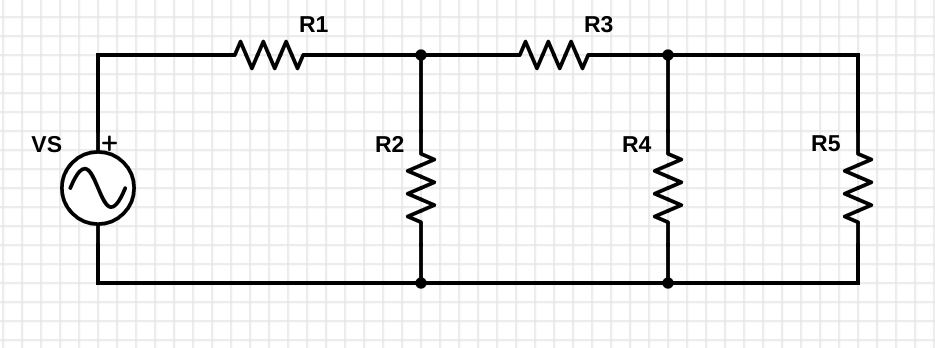
\includegraphics[scale=0.4]{images/cic1}
			\caption{Esquem�tico Circuito 1}
			\label{cic1}
		\end{figure}
		
		Para simplificar o circuito foi usado o m�todo do Equivalente de Theven�n, para o c�lculo da resist�ncia equivalente $R_{TH}$ foi usada a Equa��o \ref{rth1}.
		\begin{equation} \label{rth1}
			\begin{split}
				R_{TH}=\left[ \left(R_{1}//R_{2}\right) + R_{3}\right] // R_{4}  \\
				R_{TH}=\frac{\left[ \left( \frac{R_{1} \cdot R_{2}}{R_{1} + R_{2}} \right) + R_{3} \right] \cdot R_{4}}{\left[ \left( \frac{R_{1} \cdot R_{2}}{R_{1} + R_{2}} \right) + R_{3} + R_{4}\right]} \\
				R_{TH}=\frac{\left[ \left( R_{1} \cdot R_{2} \right) + R_{3} \cdot \left( R_{1} + R_{2} \right) \right] \cdot R_{4}}{\left( R_{1} \cdot R_{2} \right) + \left( R_{1} + R_{2} \right) \cdot \left( R_{3} + R_{4} \right)}
			\end{split}
		\end{equation}

Para o c�lculo da tens�o equivalente $V_{TH}$ foram usados dois divisores de tens�o como mostram as Equa��es \ref{vx} e \ref{vth1} e a Figura \ref{figvx}.

		\begin{figure}[htbp]
			\centering
				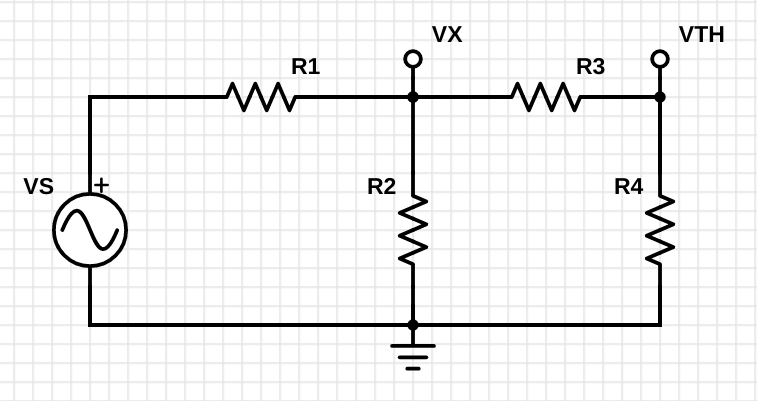
\includegraphics[scale=0.4]{images/figvx}
			\caption{Circuito para o c�lculo de $V_{TH}$}
			\label{figvx}
		\end{figure}

		\begin{equation} \label{vx}
			\begin{split}
				V_{X}=\frac{\left[\left(R_{3} + R_{4}\right)//R_{2}\right]}{\left[ \left(R_{3} + R_{4}\right)//R_{2} \right] + R_{1}} \\			
				V_{X}=\frac{\left[\frac{\left(R_{3} + R_{4}\right) \cdot R_{2}}{R_{2} + R_{3} + R_{4}}\right]}{\left[\frac{\left(R_{3} + R_{4}\right) \cdot R_{2}}{R_{2} + R_{3} + R_{4}}\right] + R_{1}} \cdot V_{S} \\
				V_{X}=\frac{\left(R_{3} + R_{4} \right) \cdot R_{2}}{\left(R_{3} + R_{4} \right) \cdot R_{2} + R_{1} \cdot \left( R_{2} + R_{3} + R_{4}\right)} \cdot V_{S} 
			\end{split}
		\end{equation}
		
		\begin{equation} \label{vth1}
			\begin{split}
				V_{TH}=\frac{R_{4}}{R_{3} + R_{4}} \cdot V_{X} \\
				V_{TH}=\frac{R_{4}}{R_{3} + R_{4}} \cdot \frac{\left(R_{3} + R_{4} \right) \cdot R_{2}}{\left(R_{3} + R_{4} \right) \cdot R_{2} + R_{1} \cdot \left( R_{2} + R_{3} + R_{4}\right)} \cdot V_{S} \\
				V_{TH}=\frac{R_{2} \cdot R_{4}}{\left(R_{3} + R_{4}\right) \cdot R_{2} + \left(R_{3} + R_{4}\right) \cdot R_{1} + R_{2}\cdot R_{1}}\cdot V_{S} \\
				V_{TH}=\frac{R_{2} \cdot R_{4}}{\left(R_{3} + R_{4}\right)\cdot\left(R_{1} + R_{2}\right) + R_{1}\cdot R_{2}} \cdot V_{S}
			\end{split}
		\end{equation}

O circuito equivalente pode ser mostrado na Figura \ref{thevenin}.

		\begin{figure}[htbp]
			\centering
				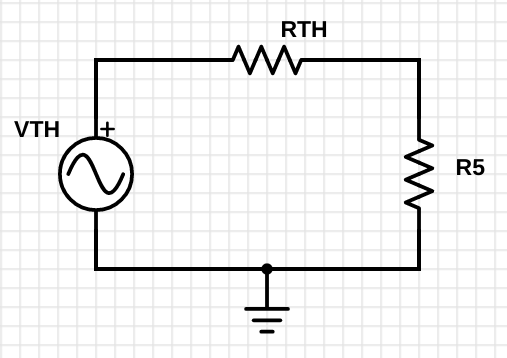
\includegraphics[scale=0.4]{images/thevenin}
			\caption{Equivalente de Theven�n}
			\label{thevenin}
		\end{figure}

Usando um divisor de tens�o � poss�vel encontrar a Equa��o \ref{vr51} que descreve a tens�o na carga $R_{5}$.

		\begin{equation} \label{vr51}
			\begin{split}
				V_{R5}=\frac{R_{5}}{R_{5} + R_{TH}} \cdot V_{TH} \\
				V_{R5}=\frac{R_{5}}{R_{5} + \frac{\left[ \left( R_{1} \cdot R_{2} \right) + R_{3} \cdot \left( R_{1} + R_{2} \right) \right] \cdot R_{4}}{\left( R_{1} \cdot R_{2} \right) + \left( R_{1} + R_{2} \right) \cdot \left( R_{3} + R_{4} \right)}} \cdot \frac{R_{2} \cdot R_{4}}{\left(R_{3} + R_{4}\right)\cdot\left(R_{1} + R_{2}\right) R_{1}\cdot R_{2}} \cdot V_{S} \\
			V_{R5}=\frac{R_{2} \cdot R_{4} \cdot R_{5}}{   R_{1} \cdot R_{2} \cdot R_{4} + R_{3} \cdot R_{4} \cdot \left( R_{1} + R_{2} \right) + R_{5}  \cdot \left( R_{1} + R_{2} \right) \cdot \left( R_{3} + R_{4} \right) + R_{1} \cdot R_{2} \cdot R_{5}   } \cdot V_{S}
			\end{split}
		\end{equation}

No experimento foram usados os valores de $R_{1}=R_{5}=56\Omega$ e $R_{2}=R_{4}=R_{5}=100\Omega$, a  Tabela \ref{s1} mostra os valores de tens�o na carga para diferentes tens�es de entrada $V_{R5}$.

\begin{table}[h!]
\centering
\caption{Valores da tens�o na carga para diferentes entradas}
\label{s1}
\begin{tabular}{l|l|l|l|}
\cline{2-4}
 & \textit{\textbf{Tens�o Cont�nua}} & \multicolumn{2}{l|}{\textit{\textbf{Tens�o Alternada}}} \\ \hline
\multicolumn{1}{|l|}{\textit{\textbf{$V_{S}$}}} & 12V & 9$V_{RMS}$ & 12.17$V_{P}$ \\ \hline
\multicolumn{1}{|l|}{\textit{\textbf{$V_{R5}$}}} & 1.60V & 1.20$V_{RMS}$ & 1.70$V_{P}$ \\ \hline
\end{tabular}
\end{table}

\subsubsection{Circuito 2}

		O circuito 2 est� representado na Figura \ref{cic2}.

		\begin{figure}[htbp]
			\centering
				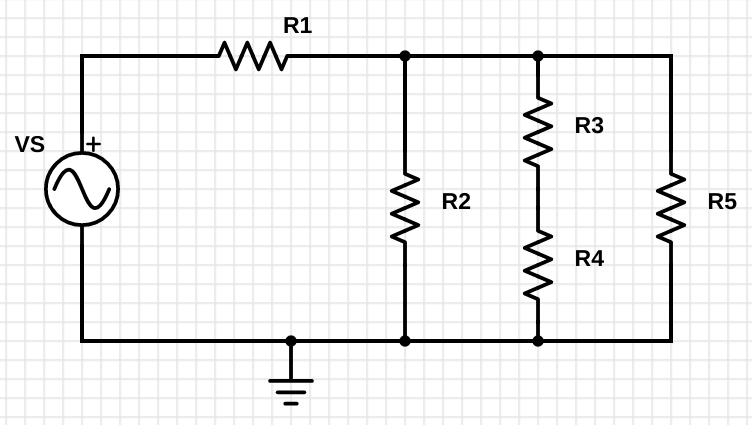
\includegraphics[scale=0.4]{images/cic2}
			\caption{Esquem�tico Circuito 2}
			\label{cic2}
		\end{figure}		

		Para simplificar o circuito foi usado o m�todo do Equivalente de Theven�n, para o c�lculo da resist�ncia equivalente $R_{TH}$ foi usada a Equa��o \ref{rth2}.
		\begin{equation} \label{rth2}
			\begin{split}
				R_{TH}=R_{1}//R_{2}//\left( R_{3} + R_{4} \right) \\
				R_{TH}=\frac{\left(\frac{R_{1}\cdot R_{2}}{R_{1} + R_{2}}\right) \cdot \left( R_{3} + R_{4} \right)}{\left(\frac{R_{1}\cdot R_{2}}{R_{1} + R_{2}}\right) + R_{3} + R_{4}} \\
				R_{TH}=\frac{R_{1} \cdot R_{2} \cdot \left( R_{3} + R_{4} \right)}{\left( R_{1} + R_{2} \right) \cdot \left( R_{3} + R_{4} \right) + R_{1} \cdot R_{2}}
			\end{split}
		\end{equation}
Para o c�lculo de $V_{TH}$ foi usado um divisor de tens�o como mostra a Equa��o \ref{vth2}.

		\begin{equation} \label{vth2}
			\begin{split}
				V_{TH}=\frac{R_{2}//\left( R_{3} + R_{4} \right)}{R_{2}//\left( R_{3} + R_{4} \right) + R_{1}} \\
				V_{TH}=\frac{\frac{R_{2}\cdot \left( R_{3} + R_{4} \right)}{R_{2} + R_{3} + R_{4}}}{\frac{R_{2}\cdot \left( R_{3} + R_{4} \right)}{R_{2} + R_{3} + R_{4}} + R_{1}} \cdot V_{S} \\
				V_{TH}=\frac{R_{2}\cdot \left( R_{3} + R_{4} \right)}{R_{2}\cdot \left( R_{3} + R_{4} \right) + R_{1}\cdot \left( R_{2} + R_{3} + R_{4} \right)}\cdot V_{S} \\
				V_{TH}=\frac{R_{2}\cdot \left( R_{3} + R_{4} \right)}{\left( R_{1} + R_{2} \right)\cdot \left( R_{3} + R_{4} \right) + R_{1} \cdot R_{2}} \cdot V_{S}
			\end{split}
		\end{equation}

O circuito equivalente pode ser mostrado na Figura \ref{thevenin}.
Usando um divisor de tens�o � poss�vel encontrar a Equa��o \ref{vr52} que descreve a tens�o na carga $R_{5}$.

		\begin{equation} \label{vr52}
			\begin{split}
				V_{R5}=\frac{R_{5}}{R_{5} + R_{TH}} \cdot V_{TH} \\
				V_{R5}=\frac{R_{5}}{R_{5} + \frac{R_{1} \cdot R_{2} \cdot \left( R_{3} + R_{4} \right)}{\left( R_{1} + R_{2} \right) \cdot \left( R_{3} + R_{4} \right) + R_{1} \cdot R_{2}}} \cdot \frac{R_{2}\cdot \left( R_{3} + R_{4} \right)}{\left( R_{1} + R_{2} \right)\cdot \left( R_{3} + R_{4} \right) + R_{1} \cdot R_{2}} \cdot V_{S} \\
				V_{R5}=\frac{R_{2} \cdot R_{5} \cdot \left( R_{3} + R_{4} \right)}{R_{1}\cdot R_{2}\cdot \left( R_{3} + R_{4} \right) + R_{5} \cdot \left[ \left( R_{1} + R_{2} \right)\cdot \left( R_{3} + R_{4} \right) + R_{1} \cdot R_{2} \right]} \cdot V_{S} \\
				V_{R5} = \frac{R_{2} \cdot R_{5}}{R_{1} \cdot R_{2} \left( 1 + \frac{R_{5}}{R_{3} + R_{4}} \right) + R_{5} \cdot \left( R_{1} + R_{2} \right)} \cdot V_{S}
			\end{split}
		\end{equation}

No experimento foram usados os valores de $R_{1}=R_{5}=56\Omega$ e $R_{2}=R_{4}=R_{5}=100\Omega$, a  Tabela \ref{s1} mostra os valores de tens�o na carga para diferentes tens�es de entrada $V_{R5}$.

\begin{table}[h!]
\centering
\caption{Valores da tens�o na carga para diferentes entradas}
\label{s1}
\begin{tabular}{l|l|l|l|}
\cline{2-4}
 & \textit{\textbf{Tens�o Cont�nua}} & \multicolumn{2}{l|}{\textit{\textbf{Tens�o Alternada}}} \\ \hline
\multicolumn{1}{|l|}{\textit{\textbf{$V_{S}$}}} & 12V & 9$V_{RMS}$ & 12.17$V_{P}$ \\ \hline
\multicolumn{1}{|l|}{\textit{\textbf{$V_{R5}$}}} & 4.23V & 2.99$V_{RMS}$ & 4.48$V_{P}$ \\ \hline
\end{tabular}
\end{table}

\subsection{Procedimento Experimental}
Os dois circuitos foram combinados em um s� com o uso de uma chave interruptora e montados de acordo com o diagrama da Figura \ref{diagram1} para corrente cont�nua e de acordo com o diagrama da Figura \ref{diagram2} para corrente alternada na bancada como mostra a Figura \ref{cicban} e foram medidas as tens�es na carga $R_{5}$.

		\begin{figure}[htbp]
			\centering
				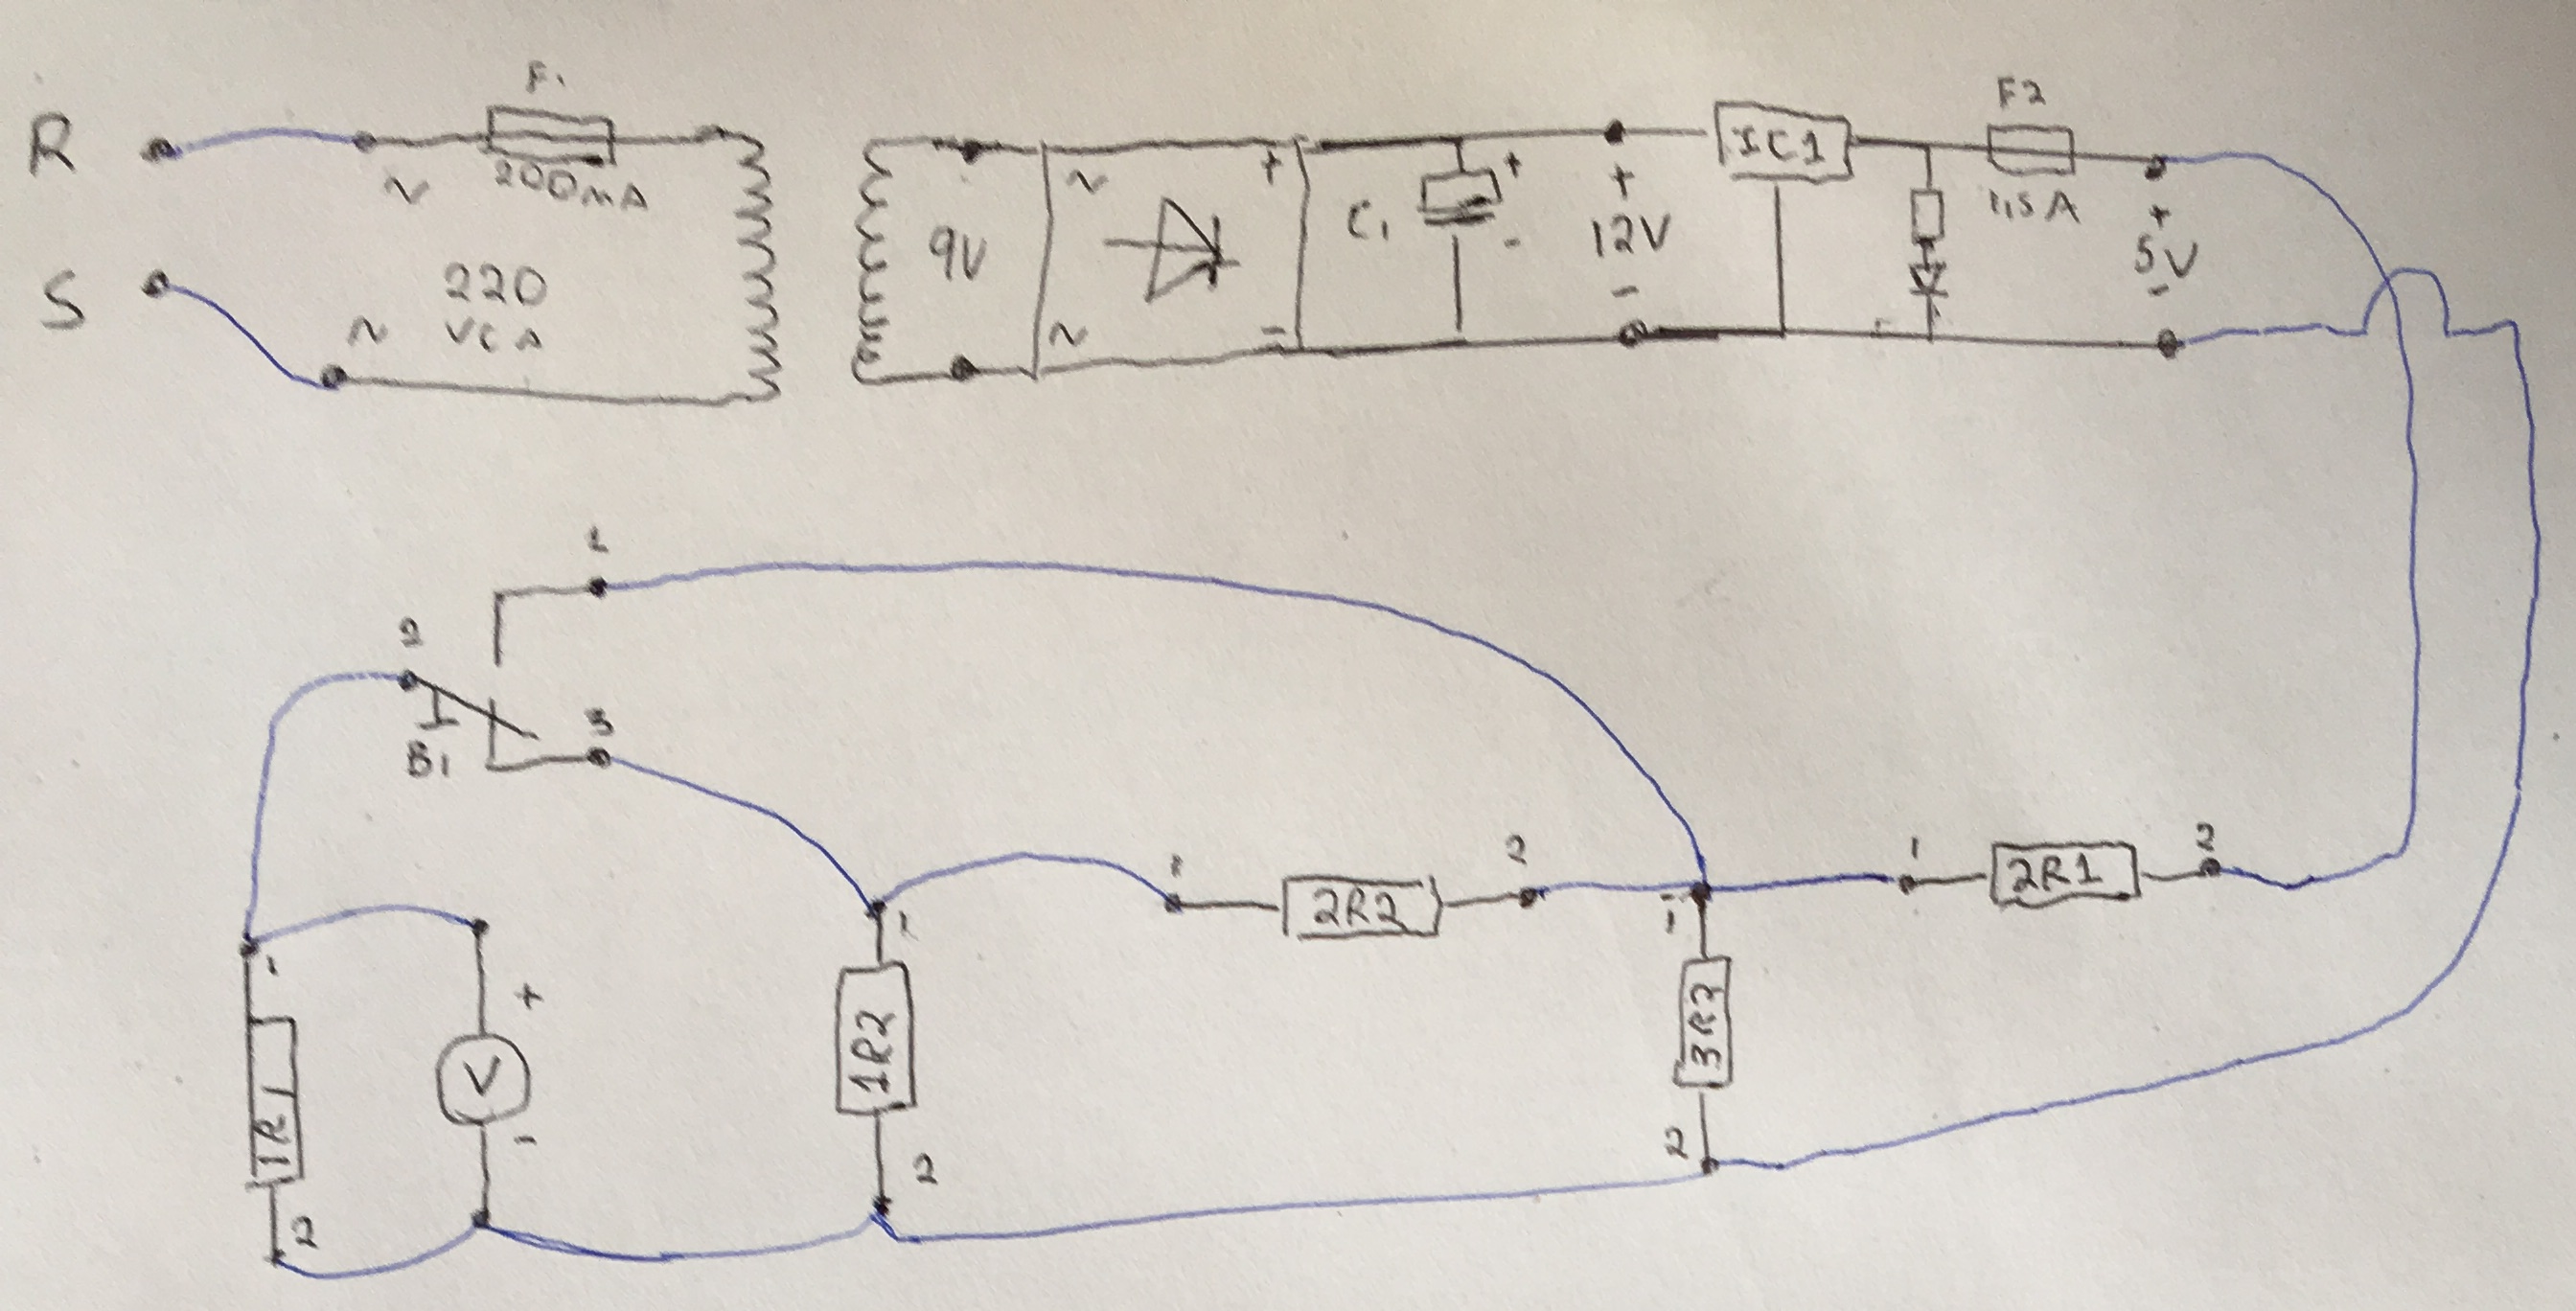
\includegraphics[scale=0.12]{images/diagram1.png}
			\caption{Diagrama de Montagem DC} 
			\label{diagram1}
		\end{figure}

		\begin{figure}[htbp]
			\centering
				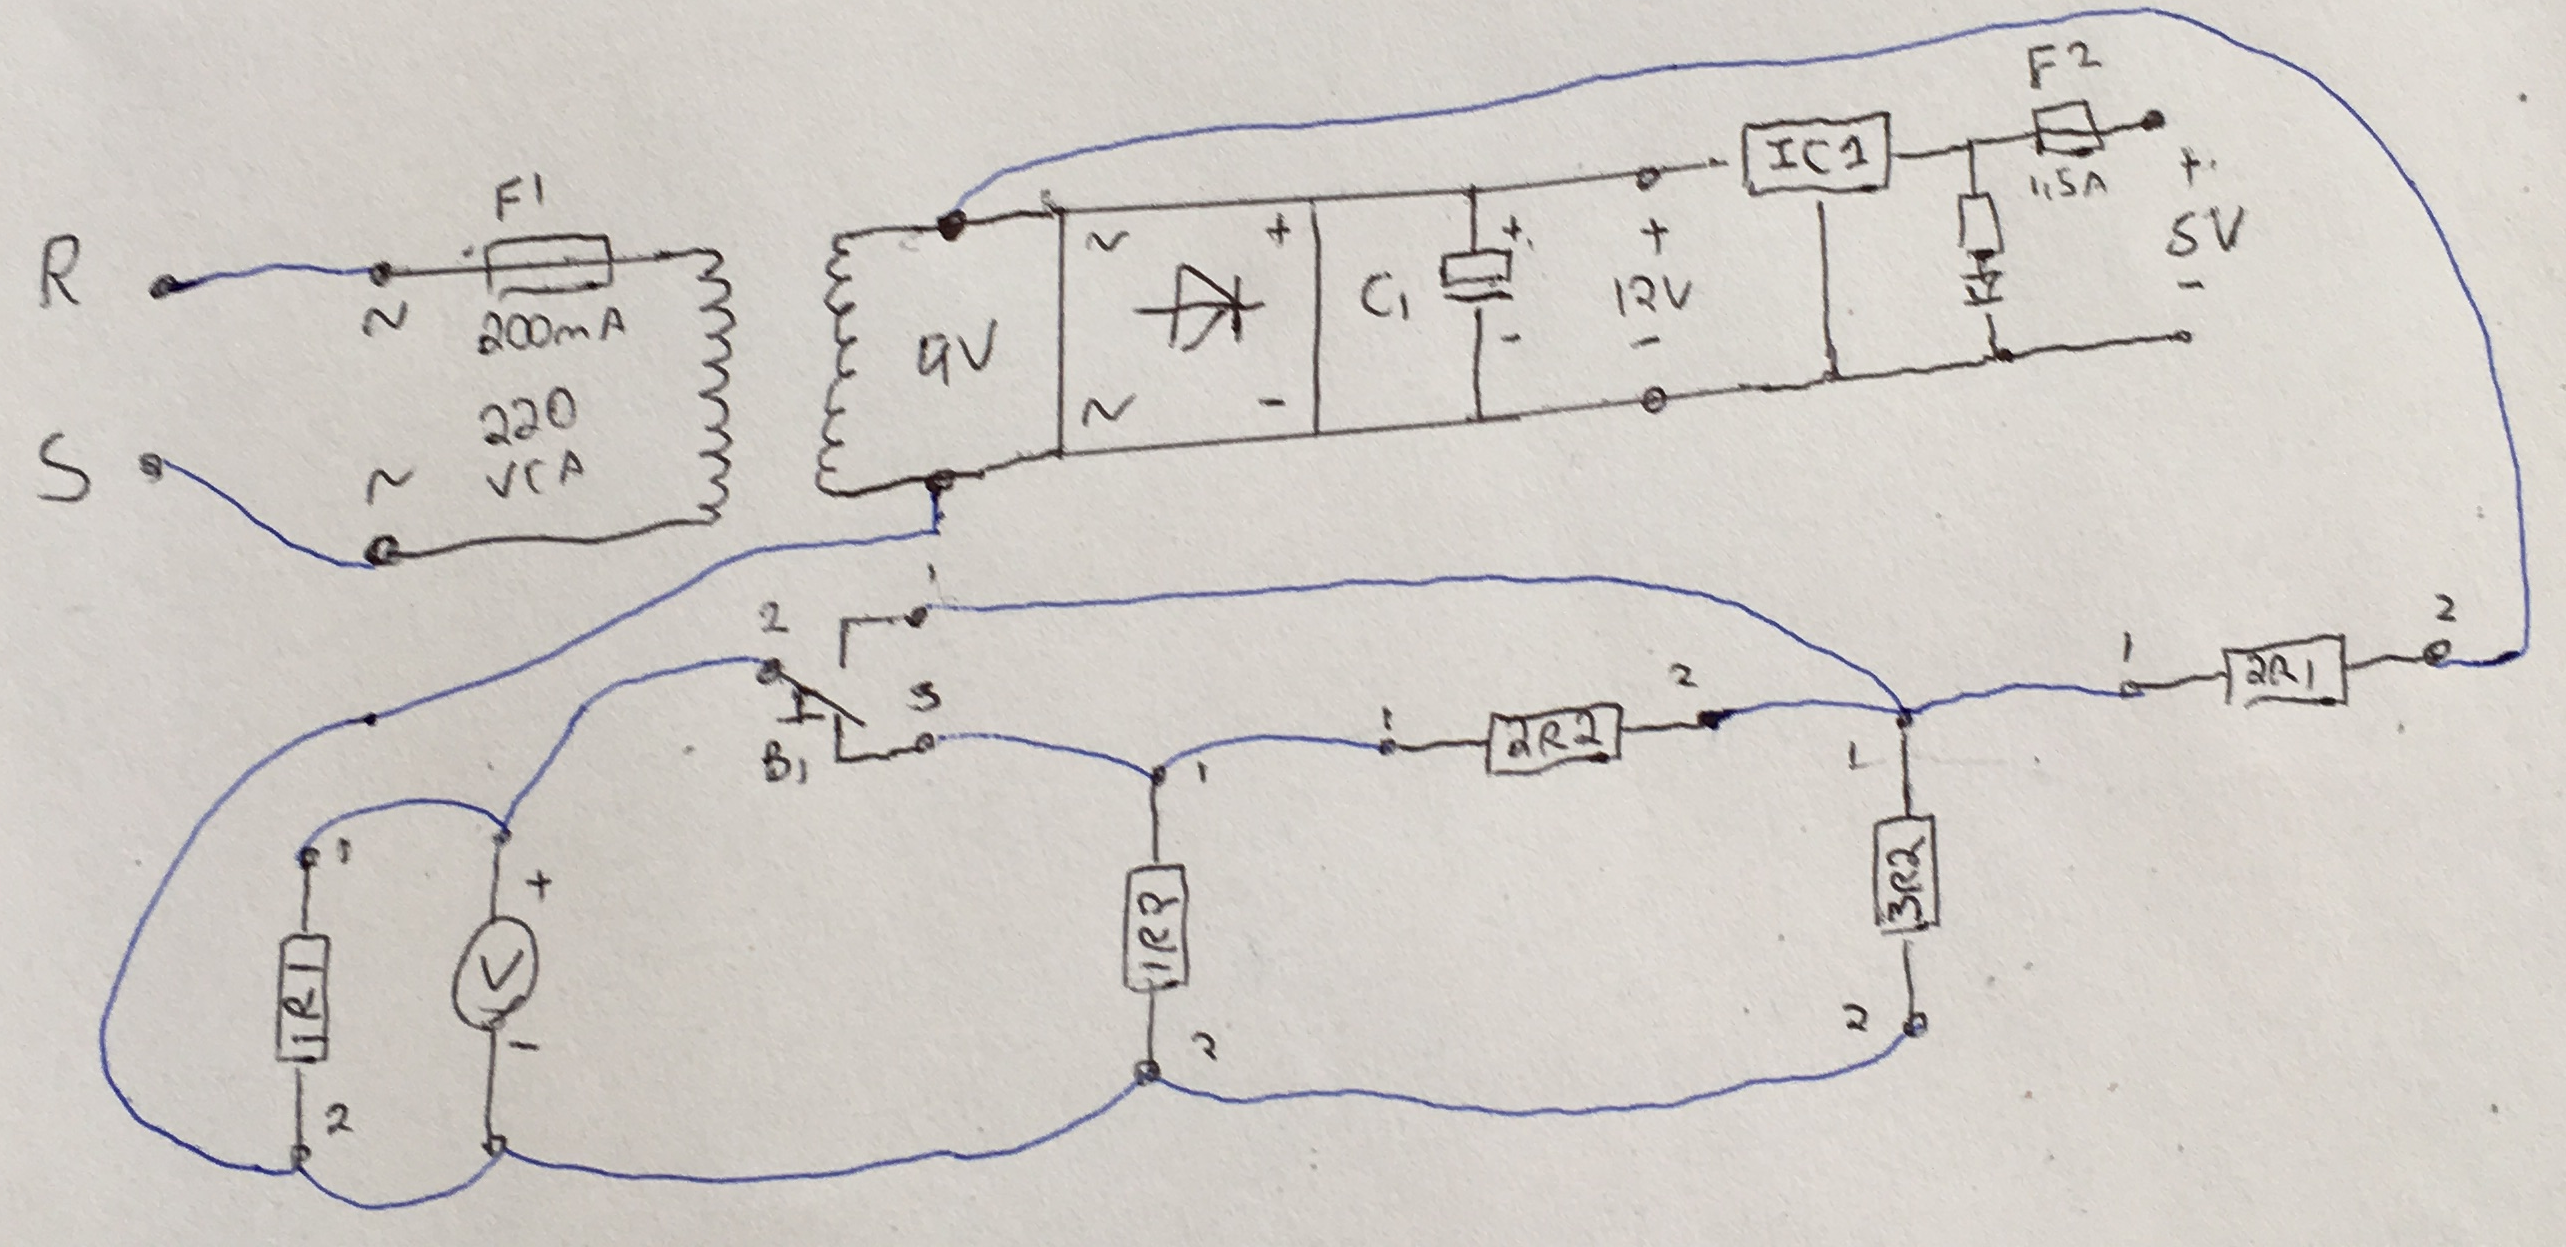
\includegraphics[scale=0.15]{images/diagram2.png}
			\caption{Diagrama de Montagem AC}
			\label{diagram2}
		\end{figure}

		\begin{figure}[htbp]
			\centering
				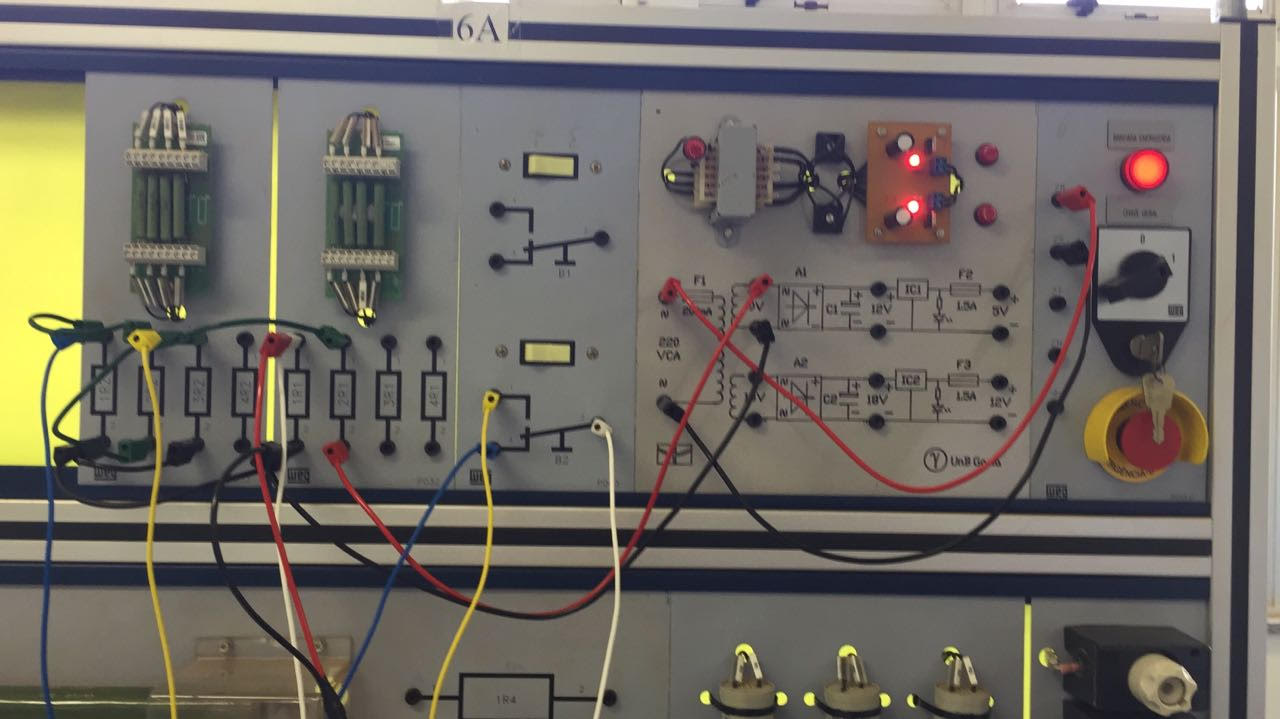
\includegraphics[scale=0.35]{images/cicban.png}
			\caption{Circuitos montados na bancada}
			\label{cicban}
		\end{figure}

\section{Resultados} 
Os resultados da primeira parte do experimento, o calculo dos par�metros de imped�ncia dos quadripolos das figuras XX e XX, est�o registrados nas quatro tabelas a seguir:

\section{Discuss�o e Conclus�es}
Os valores te�ricos usados nas analises dos resultados desse experimento foram obtidos  atrav�s de c�lculos te�ricos usando o software de simula��o QUCS para confirmar o c�lculos. Sabe-se que em um ambiente experimental existem muitas outras vari�veis, algumas conhecidas outras n�o, que afetam o comportamento do circuito. Porem ainda com essas diferen�as no experimento todos os valores obtidos est�o de acordo com a analise te�rica. O experimento foi um sucesso pois os valores experimentais foram concisos com a teoria e apos a realiza��o da experiencia foi poss�vel compreender melhor os par�metros de imped�ncia, admit�ncia e transmiss�o e a import�ncia deles para associa��o de quadripolo.


\small
% IEEEtran is a LaTeX style file defining the reference formatting.
% -----------------------------------------------------------------
\bibliographystyle{IEEEtran}
\bibliography{fixos/IEEEabrv,fixos/labrefs}
%\bibliography{IEEEabrv,fpl_refs}


\end{document}
